%package list
\documentclass{article}
\usepackage[top=3cm, bottom=3cm, outer=3cm, inner=3cm]{geometry}
\usepackage{multicol}
\usepackage{graphicx}
\usepackage{url}
\usepackage{hyperref}
\usepackage{array}
\newcolumntype{x}[1]{>{\centering\arraybackslash\hspace{0pt}}p{#1}}
\usepackage{natbib}
\usepackage{pdfpages}
\usepackage{multirow}
\usepackage[normalem]{ulem}
\useunder{\uline}{\ul}{}
\usepackage{svg}
\usepackage{xcolor}
\usepackage{listings}
\lstdefinestyle{ascii-tree}{
    literate={├}{|}1 {─}{--}1 {└}{+}1 
  }
\lstset{basicstyle=\ttfamily,
  showstringspaces=false,
  commentstyle=\color{red},
  keywordstyle=\color{blue}
}
%\usepackage{booktabs}
\usepackage{caption}
\usepackage{subcaption}
\usepackage{float}
\usepackage{array}

% Comment
\usepackage{verbatim}

\newcolumntype{M}[1]{>{\centering\arraybackslash}m{#1}}
\newcolumntype{N}{@{}m{0pt}@{}}


%%%%%%%%%%%%%%%%%%%%%%%%%%%%%%%%%%%%%%%%%%%%%%%%%%%%%%%%%%%%%%%%%%%%%%%%%%%%
%%%%%%%%%%%%%%%%%%%%%%%%%%%%%%%%%%%%%%%%%%%%%%%%%%%%%%%%%%%%%%%%%%%%%%%%%%%%
\newcommand{\itemEmail}{rzapata@unsa.edu.pe}
\newcommand{\itemStudent}{Reyser Julio Zapata Butron}
\newcommand{\itemCourse}{Análisis Y Diseño de Algoritmos}
\newcommand{\itemCourseCode}{1702231}
\newcommand{\itemSemester}{IV}
\newcommand{\itemUniversity}{Universidad Nacional de San Agustín de Arequipa}
\newcommand{\itemFaculty}{Facultad de Ingeniería de Producción y Servicios}
\newcommand{\itemDepartment}{Departamento Académico de Ingeniería de Sistemas e Informática}
\newcommand{\itemSchool}{Escuela Profesional de Ingeniería de Sistemas}
\newcommand{\itemAcademic}{2024 - B}
\newcommand{\itemInput}{26 noviembre 2024}
\newcommand{\itemOutput}{26 noviembre 2024}
\newcommand{\itemPracticeNumber}{07}
\newcommand{\itemTheme}{Algoritmos para Grafos: Accesibilidad}
\newcommand{\itemPracticeDuration}{02 horas}
%%%%%%%%%%%%%%%%%%%%%%%%%%%%%%%%%%%%%%%%%%%%%%%%%%%%%%%%%%%%%%%%%%%%%%%%%%%%
%%%%%%%%%%%%%%%%%%%%%%%%%%%%%%%%%%%%%%%%%%%%%%%%%%%%%%%%%%%%%%%%%%%%%%%%%%%%

\usepackage[english,spanish]{babel}
\usepackage[utf8]{inputenc}
\AtBeginDocument{\selectlanguage{spanish}}
\renewcommand{\figurename}{Figura}
\renewcommand{\refname}{Referencias}
\renewcommand{\tablename}{Tabla} %esto no funciona cuando se usa babel
\AtBeginDocument{%
	\renewcommand\tablename{Tabla}
}

\usepackage{fancyhdr}
\pagestyle{fancy}
\fancyhf{}
\setlength{\headheight}{30pt}
\renewcommand{\headrulewidth}{1pt}
\renewcommand{\footrulewidth}{1pt}
\fancyhead[L]{\raisebox{-0.2\height}{
\includegraphics[width=3cm]{img/logo_episunsa.png}}}
\fancyhead[C]{\fontsize{7}{7}\selectfont	\itemUniversity \\ \itemFaculty \\ \itemDepartment \\ \itemSchool \\ \textbf{\itemCourse}}
\fancyhead[R]{\raisebox{-0.2\height}{
\includegraphics[width=1.2cm]{img/logo_abet}}}
\fancyfoot[L]{Reyser Julio Zapata Butrón}
\fancyfoot[C]{\itemCourse}
\fancyfoot[R]{Página \thepage}

% Estilos del Código
\usepackage{listings}
\usepackage{color, colortbl}
\definecolor{dkgreen}{rgb}{0,0.6,0}
\definecolor{gray}{rgb}{0.5,0.5,0.5}
\definecolor{codebackground}{rgb}{89, 0.97, 0.90}
\definecolor{tablebackground}{rgb}{0.8, 0, 0}

\lstset{
  language=C++,                  
  basicstyle=\ttfamily\footnotesize,
  keywordstyle=\color{blue},     
  commentstyle=\color{dkgreen},    
  stringstyle=\color{red},       
  backgroundcolor= \color{codebackground},
  numbers=left,                  
  numberstyle=\tiny\color{gray},
  stepnumber=1,                  
  numbersep=5pt,                
  showspaces=false,              
  showstringspaces=false,      
  showtabs=false,                
  frame=single,                  
  captionpos=b,                  %
}

\begin{document}
	\vspace*{10px}
	
	\begin{center}	
		\fontsize{17}{17} \textbf{ Informe de Laboratorio \itemPracticeNumber}
	\end{center}

 %% TABLA %%
 
	\centerline{\textbf{\Large Tema: \itemTheme}}

	\begin{flushright}
		\begin{tabular}{|M{2.5cm}|N|}
			\hline 
			\rowcolor{tablebackground}
			\color{white} \textbf{Nota}  \\
			\hline 
			     \\[30pt]
			\hline 			
		\end{tabular}
	\end{flushright}	

	\begin{table}[H]
		\begin{tabular}{|x{4.7cm}|x{4.8cm}|x{4.8cm}|}
			\hline 
			\rowcolor{tablebackground}
			\color{white} \textbf{Estudiante} & \color{white}\textbf{Escuela}  & \color{white}\textbf{Asignatura}   \\
			\hline 
			{\itemStudent \par \itemEmail} & \itemSchool & {\itemCourse \par Semestre: \itemSemester \par Código: \itemCourseCode}     \\
			\hline 			
		\end{tabular}
	\end{table}		
	
	\begin{table}[H]
		\begin{tabular}{|x{4.7cm}|x{4.8cm}|x{4.8cm}|}
			\hline 
			\rowcolor{tablebackground}
			\color{white}\textbf{Laboratorio} & \color{white}\textbf{Tema}  & \color{white}\textbf{Duración}   \\
			\hline 
			\itemPracticeNumber & \itemTheme & \itemPracticeDuration   \\
			\hline 
		\end{tabular}
	\end{table}
	
	\begin{table}[H]
		\begin{tabular}{|x{4.7cm}|x{4.8cm}|x{4.8cm}|}
			\hline 
			\rowcolor{tablebackground}
			\color{white}\textbf{Semestre académico} & \color{white}\textbf{Fecha de inicio}  & \color{white}\textbf{Fecha de entrega}   \\
			\hline 
			\itemAcademic & \itemInput &  \itemOutput  \\
			\hline 
		\end{tabular}
	\end{table}

 %% CONTENIDO %%
\section{Código base}
    El siguiente código presentado, es la base para la realización de los ejerción propuestos, añadiendo los métodos requeridos. \\
    \lstinputlisting[language=C++, caption={base.cpp}, numbers=left]{src/base.cpp}

\section{Ejercicios Propuestos}
    \subsection{Permutación de vecinos. Repite los ejemplos C y D anteriores suponiendo que el grafo G está representado por las listas de adyacencia:
            \[
            \begin{array}{r|l}
            0 & 2 \ 3 \ 4 \\
            1 & \\
            2 & 1 \ 4 \\
            3 & 4 \ 5 \\
            4 & 1 \ 5 \\
            5 & 1 \\
            \end{array}
            \]
    }

        \lstinputlisting[language=C++, caption={exercise1.cpp}, numbers=left]{src/exercise1.cpp}

        \textbf{Ejecución del código}
            \begin{figure}[H]
            	\centering
             	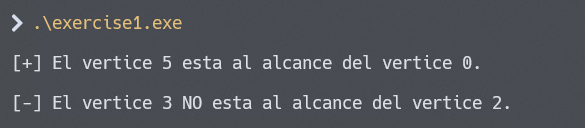
\includegraphics[width=0.8\textwidth,keepaspectratio]{img/exercise1.png}
            \end{figure}

        \subsubsection*{Explicación del Código}
            El código implementa una búsqueda en un grafo \textbf{dirigido} utilizando el algoritmo de búsqueda en profundidad (DFS). La estructura del grafo está representada por una matriz de adyacencia, donde un valor de 1 indica la existencia de un arco dirigido entre dos vértices. La función \texttt{GRAPHreach} recibe dos vértices \( s \) y \( t \), y determina si hay un camino dirigido entre ellos.
            
        \subsubsection*{Funcionamiento}
           1. \textbf{Inicialización:} La función \texttt{GRAPHreach} inicializa el vector \texttt{visited[]} para marcar los vértices visitados durante la búsqueda. Luego, llama a la función recursiva \texttt{reachR} comenzando desde el vértice \( s \).
   
            2. \textbf{Búsqueda recursiva (DFS):} La función \texttt{reachR} recorre los vértices adyacentes al vértice \( v \) y, si un vértice adyacente no ha sido visitado, realiza una llamada recursiva para continuar la búsqueda.
            
            3. \textbf{Determinación del camino:} Si durante la búsqueda el vértice \( t \) es alcanzado, la función \texttt{GRAPHreach} retorna \texttt{true}, indicando que \( t \) está al alcance de \( s \). De lo contrario, retorna \texttt{false}.

            
        \subsubsection*{Complejidad Temporal}
            La complejidad temporal del algoritmo es \( O(V + E) \), donde \( V \) es el número de vértices y \( E \) es el número de arcos. Esto se debe a que cada vértice es visitado una sola vez, y cada arco es examinado una vez.


    \subsection{Versión ansiosa de la función. Escriba una variante de la función GRAPHreach() que se detenga inmediatamente (y devuelva true) al descubrir que t está al alcance de s. (El código de reachR() para esta variante es más complicado que el de la versión ansiosa discutida anteriormente). Para hacer el ejercicio más interesante, imprime un camino de s a t antes de devolver true.}

        \lstinputlisting[language=C++, caption={exercise2.cpp}, numbers=left]{src/exercise2.cpp}

        \textbf{Ejecución del código}
            \begin{figure}[H]
            	\centering
             	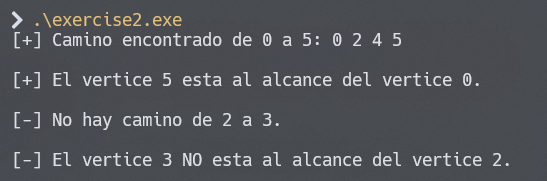
\includegraphics[width=0.8\textwidth,keepaspectratio]{img/exercise2.png}
            \end{figure}

        \subsubsection*{Explicación de los Cambios en el Código}
            En este ejercicio, la función \texttt{GRAPHreach()} fue modificada para detenerse inmediatamente después de encontrar el vértice \( t \) y para imprimir el camino de \( s \) a \( t \). A continuación se explican los cambios con fragmentos de código.
            
        \subsubsection*{Función \texttt{GRAPHreach()}}
            La principal modificación en esta función es que ahora se imprime el camino de \( s \) a \( t \) si se encuentra un camino, y la función se detiene de inmediato al encontrar \( t \).
            
            \begin{verbatim}
            bool GRAPHreach(Graph &G, vertex s, vertex t) {
                for (vertex v = 0; v < G.V; ++v)
                    visited[v] = 0;
                path.clear();  // Se limpia el vector de camino
            
                if (reachR(G, s, t)) {
                    cout << "[+] Camino encontrado de " << s << " a " << t << ": ";
                    for (vertex v : path)  // Imprime el camino
                        cout << v << " ";
                    cout << endl;
                    return true;
                } else {
                    cout << "\n[-] No hay camino de " << s << " a " << t << "." << endl;
                    return false;
                }
            }
            \end{verbatim}

        Aquí, si la función \texttt{reachR()} retorna \texttt{true}, se imprime el camino almacenado en el vector \texttt{path[]}.

        \subsubsection*{Función \texttt{reachR()}} 
            La función \texttt{reachR()} fue modificada para que, en cuanto se encuentre el vértice \( t \), se devuelva \texttt{true} inmediatamente, y el vértice actual se agregue a \texttt{path[]}. Además, si el vértice \( t \) no es alcanzado por el camino actual, se elimina el vértice de \texttt{path[]}.
            
            \begin{verbatim}
            static bool reachR(Graph &G, vertex v, vertex t) {
                visited[v] = 1;        // Marca el vértice como visitado
                path.push_back(v);     // Agrega el vértice al camino
            
                if (v == t)            // Si encontramos el vértice t
                    return true;
            
                for (vertex w = 0; w < G.V; ++w) {
                    if (G.adj[v][w] == 1 && visited[w] == 0) {
                        if (reachR(G, w, t))  // Llamada recursiva
                            return true;
                    }
                }
            
                path.pop_back();  // Si no encontramos t, deshacemos el último paso
                return false;
            }
            \end{verbatim}

        Las modificaciones clave son:
            \begin{itemize}
                \item \texttt{path.push\_back(v)}: Añade el vértice \( v \) al camino.
                \item \texttt{if (v == t)}: Si el vértice actual es \( t \), se retorna \texttt{true} y el camino es impreso.
                \item \texttt{path.pop\_back()}: Si no se encuentra un camino hacia \( t \), el vértice actual se elimina de \texttt{path[]}.
            \end{itemize}
 
%%% REPOSITORIO DE GITHUB %%%
\section{Repositorio de Github}
	\begin{itemize}
		\item Repositorio de Github donde se encuentra el actual laboratorio \\
		\url{https://github.com/ReyserLynnn/ada-lab-b-24b/tree/main/laboratorio07/src}

        \item Repositorio de Github donde se encuentran los laboratorios del curso\\
		\url{https://github.com/ReyserLynnn/ada-lab-b-24b.git}
	\end{itemize}

\section{Conclusión}
En este laboratorio, aprendí a trabajar con algoritmos de búsqueda en grafos, usando recursión y una versión más eficiente que se detiene al encontrar el destino. También entendí cómo seguir el camino y mostrarlo, evitando seguir explorando una vez que ya encontré lo que buscaba.
    

\begin{comment}
\section{Referencias}
\begin{itemize}			
	\item \url{https://dialnet.unirioja.es/servlet/articulo?codigo=4573315}
\end{itemize}	    
\end{comment}

\end{document}